% !TEX root = comparison.tex

\subsection{Comparing Distributions}
\begin{figure*}[htbp] %  figure placement: here, top, bottom, or page
   \centering
   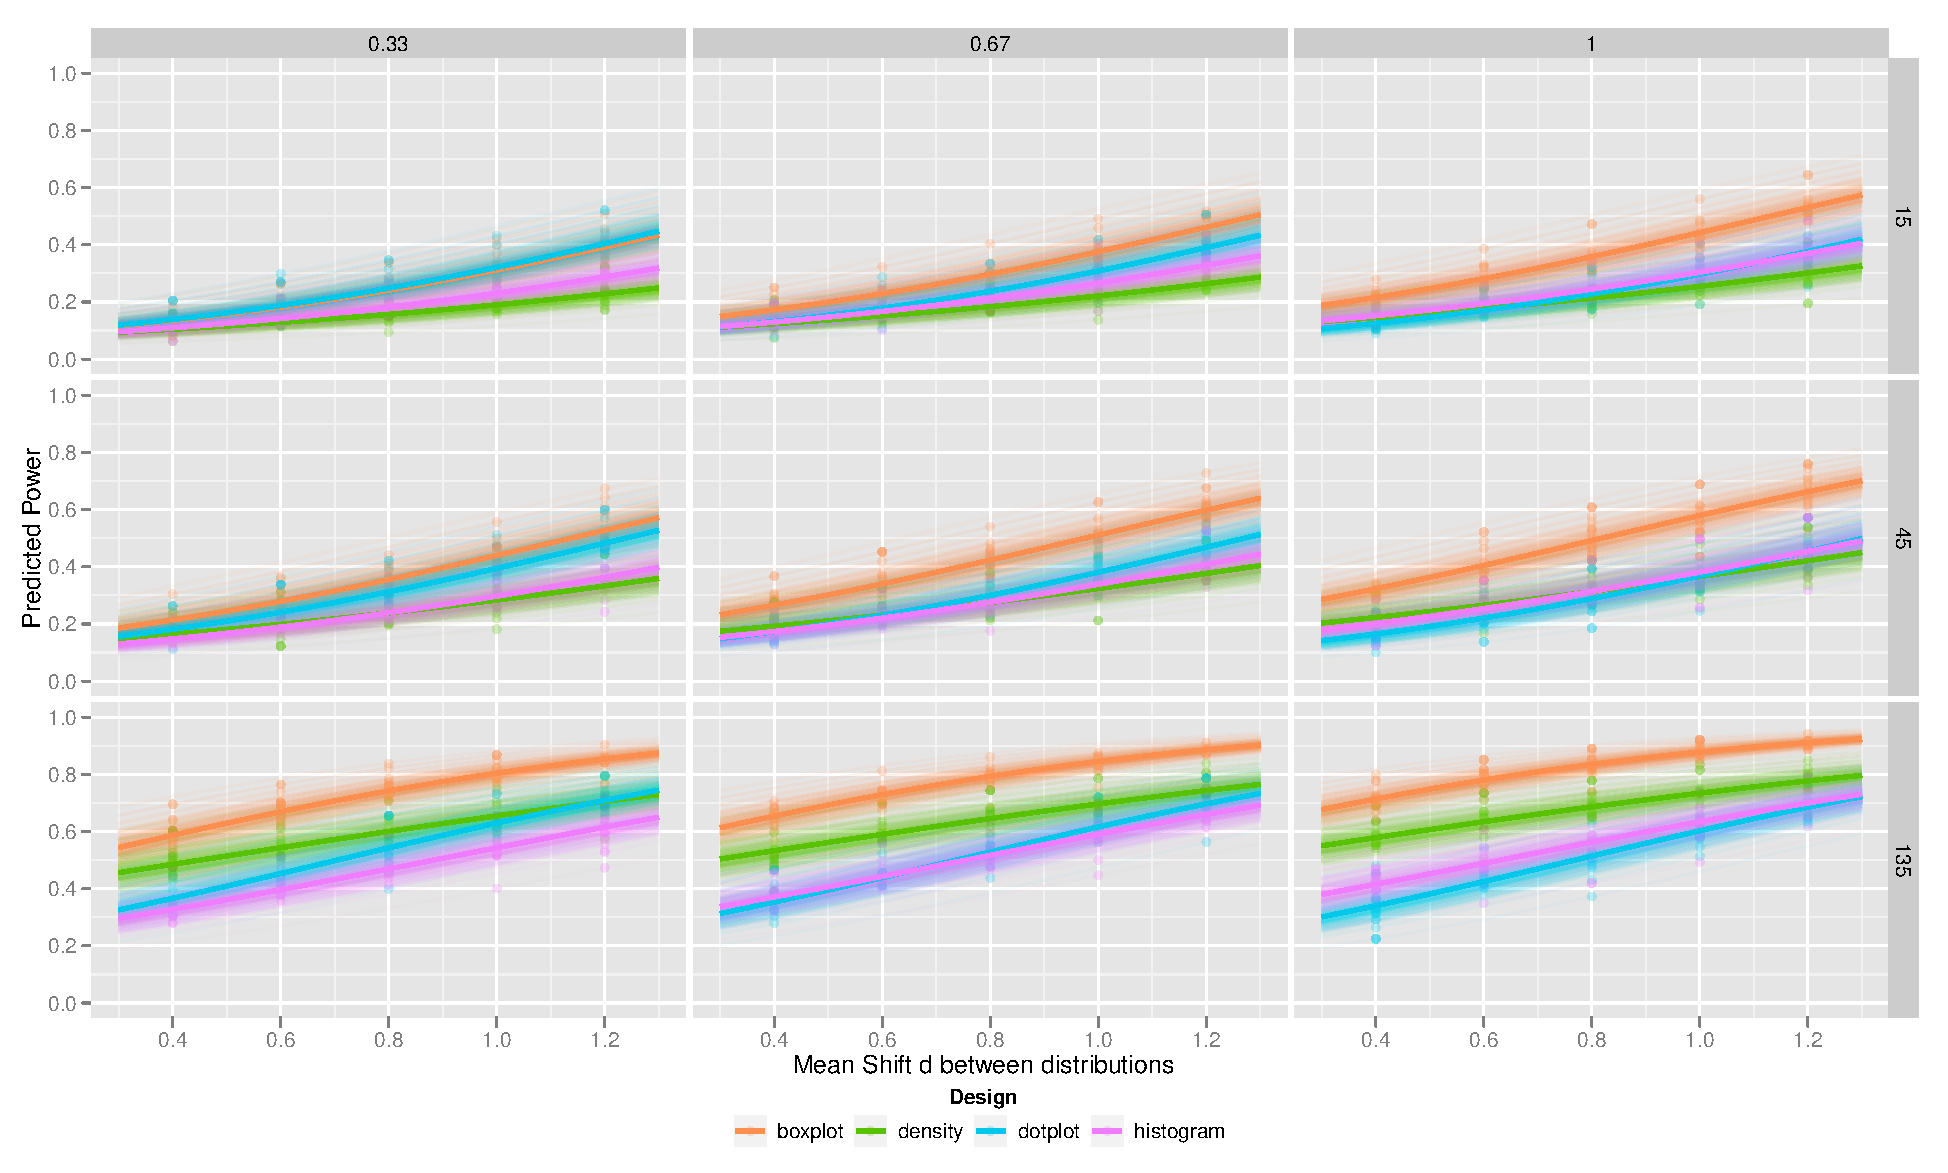
\includegraphics[width=\linewidth]{power-exp2} 
   \caption{Overview of power predictions for the four different designs. The fully saturated thick lines show average predicted power for each of the designs facetted by size of the red group (top to bottom) and relative size of the blue group to the red group (left to right). }
   \label{fig:power2}
\end{figure*}

Since each participant provides results from nine lineups, we can use a generalized linear mixed effects model of power and account for individuals' abilities by including a subject-specific random intercept. We included all of the above described covariates  in the model, both as main effects and as two-way interaction with the design to assess their impact on the power of each of the designs.
Figure \ref{fig:power2} summarizes the modeling results as shown in table \ref{tbl:power2}. Generally we can see that the power of all four designs increases with an increase in effect size ($x$ axis), as well as an increase in sample size (top to bottom facetting). Depending on visualization setup, different designs have highest power: boxplots  are an alround good choice in visualizing a mean shift in a distribution. For small overall sample size dotplots (green dots and lines) show good power, but they  start to lose their advantage in favor of more summarized plots, such as density charts or histograms. Following the predicted power for density charts for the different ratios between the groups, we see that from left to right the density line does not benefit from additional information in the second group, unlike all of the other designs. Dotplots are the only design, in which each observation is shown individually. This increase in visual complexity might be the reason behind this phenomenon.

Density charts profit the most from an increase in sample size - making them particularly good design choices for a larger sample sizes.
\begin{table}[ht]
\begin{center}
\begin{tabular}{rrrrr}
  \hline
 & Estimate & Std. Error & $z$ value & $p$-value \\ 
  \hline
(Intercept) & -3.11 & 0.41 & -7.61 & 0.00 \\ 
  density & 0.05 & 0.57 & 0.09 & 0.93 \\ 
  dotplot & 0.46 & 0.57 & 0.81 & 0.42 \\ 
  histogram & 0.06 & 0.58 & 0.11 & 0.91 \\ 
  d & 1.77 & 0.34 & 5.18 & 0.00 \\ 
  n1 & 0.02 & 0.00 & 9.73 & 0.00 \\ 
  ratio & 0.84 & 0.33 & 2.56 & 0.01 \\ 
  density:d & -0.60 & 0.47 & -1.27 & 0.20 \\ 
  dotplot:d & 0.03 & 0.46 & 0.07 & 0.95 \\ 
  histogram:d & -0.28 & 0.48 & -0.59 & 0.56 \\ 
  density:n1 & -0.00 & 0.00 & -0.36 & 0.72 \\ 
  dotplot:n1 & -0.01 & 0.00 & -3.00 & 0.00 \\ 
  histogram:n1 & -0.01 & 0.00 & -2.64 & 0.01 \\ 
  density:ratio & -0.28 & 0.47 & -0.59 & 0.56 \\ 
  dotplot:ratio & -1.01 & 0.46 & -2.19 & 0.03 \\ 
  histogram:ratio & -0.28 & 0.47 & -0.59 & 0.55 \\ 
   \hline
\end{tabular}
\end{center}
\caption{Results from a Generalized Linear Mixed Effects Model of Power of a lineup given design and all two-way interactions with effect size $d$, group size $n_1$, and ratio to second to first group size. The model was fit based on 2513 lineup evaluations of 208 participants.}
\label{tbl:power2}
\end{table}

\begin{table}[ht]
\begin{center}
\begin{tabular}{rrrrr}
  \hline
 & Estimate & Std..Error & t.value & pval \\ 
  \hline
(Intercept) & 3.85 & 0.09 & 42.21 & 0.00 \\ 
  density & 0.01 & 0.12 & 0.07 & 0.94 \\ 
  dotplot & 0.03 & 0.12 & 0.26 & 0.80 \\ 
  histogram & 0.23 & 0.12 & 1.97 & 0.05 \\ 
  d & -0.23 & 0.08 & -3.02 & 0.00 \\ 
  n1 & 0.00 & 0.00 & 1.74 & 0.08 \\ 
  I(n1/n2) & -0.04 & 0.02 & -1.48 & 0.14 \\ 
  density:d & 0.11 & 0.11 & 1.02 & 0.31 \\ 
  dotplot:d & 0.20 & 0.11 & 1.86 & 0.06 \\ 
  histogram:d & -0.01 & 0.11 & -0.09 & 0.93 \\ 
  density:n1 & -0.00 & 0.00 & -2.15 & 0.03 \\ 
  dotplot:n1 & -0.00 & 0.00 & -2.87 & 0.00 \\ 
  histogram:n1 & -0.00 & 0.00 & -0.93 & 0.35 \\ 
  density:I(n1/n2) & 0.04 & 0.03 & 1.18 & 0.24 \\ 
  dotplot:I(n1/n2) & 0.02 & 0.03 & 0.65 & 0.52 \\ 
  histogram:I(n1/n2) & 0.00 & 0.04 & 0.04 & 0.97 \\ 
   \hline
\end{tabular}
\end{center}
\caption{log time taken}

\end{table}



